\chapter{Evaluation results}
This section will give an overview of the raw results gathered by the evaluations performed on the different prototypes.
\section{Capacitive chair posture recognition - manual classifier}
This section provides raw data of the first posture recognition test performed using the capacitive chair. 
\subsection{Evaluation setup}
Short study with 10 participants. Three poses and a non-pose:
\begin{itemize}
\item Sitting upright
\item Sitting hunched
\item Slouching on chair
\item Close to chair - disturber
\end{itemize}

The persons were given a short introduction, the different postures were displayed, and finally the persons were asked to perform the postures in order. When testing “close-to-chair” the subjects were asked to rattle at the chair, stand close, move it around and thus disturb the potential sensor readings. Each class was tested for 10 seconds, collecting 200 samples. 

\subsection{Raw results}
\begin{table}[htbp]
  \centering
  \caption{Percentage of correctly classified postures using manually set classifier}
    \begin{tabularx}{\linewidth}{XXXXXXXXXXXX}
    \toprule
          & S1    & S2    & S3    & S4    & S5    & S6    & S7    & S8    & S9    & S10   & Avg \\
    \midrule
    Upright & 100   & 100   & 100   & 100   & 100   & 100   & 100   & 100   & 100   & 100   & 100 \\
    Hunched & 100   & 100   & 100   & 100   & 86    & 100   & 100   & 100   & 100   & 100   & 98,6 \\
    Slouch & 100   & 100   & 100   & 100   & 100   & 100   & 100   & 100   & 55    & 100   & 95,5 \\
    Disturber & 100   & 100   & 100   & 100   & 100   & 100   & 100   & 100   & 100   & 100   & 100 \\
    \bottomrule
    \end{tabularx}%
  \label{tab:app_eval_chair_raw1}%
\end{table}%
\subsection{Postures}
\begin{figure}[h]
\centering
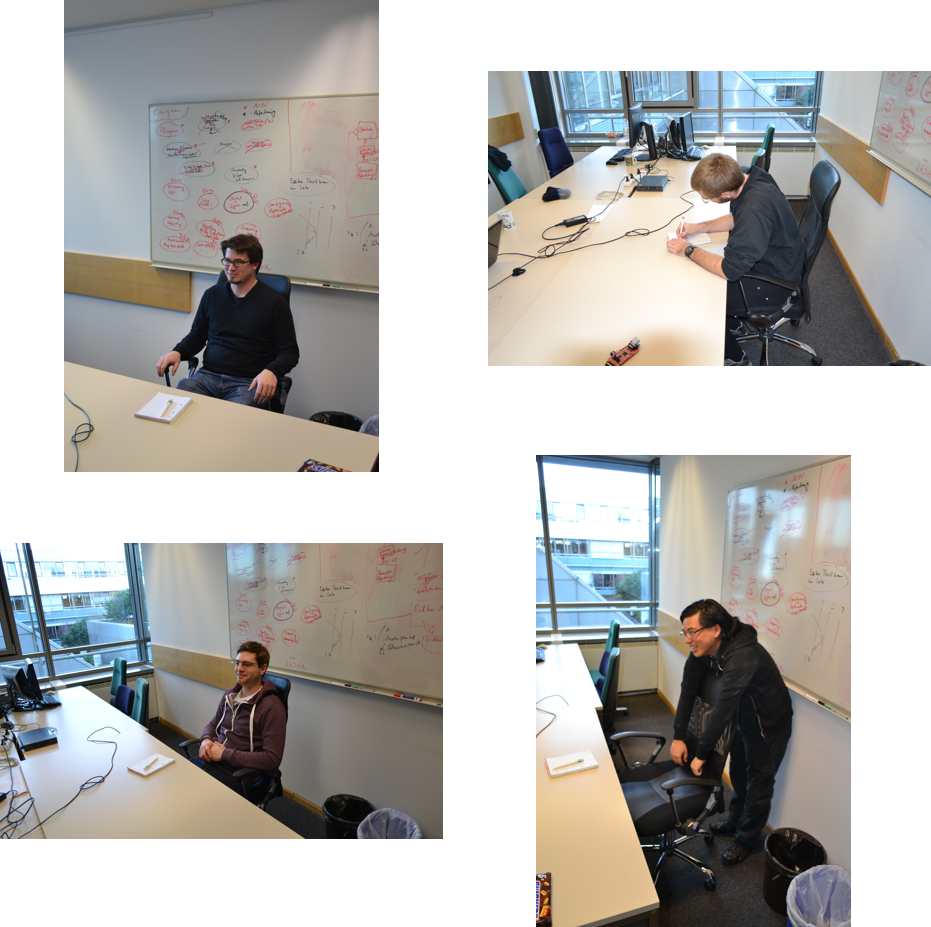
\includegraphics[width=0.8\textwidth]{images/app_eval_chair1}
\caption{\emph{Top left} upright posture. \emph{Top right} hunched posture. \emph{Bottom left} slouched posture. \emph{Bottom right} disturber posture}
\label{fig:disc_unob_elec}
\end{figure}




